\section{Methodology}
\label{sec:overview} 

This section outlines the methodology we will use for our experiments.
We will use a set of ninety-seven apps applications during testing, using
automated experiments to analyze each and every one. Finally, the results
of these experiments will be analyzed for any true and/or false vulnerabilites
present within each app.

\subsection{Set of Apps}

We have been given a set of ninety-seven .apk applications to test, many of 
which contain different purposes, uses, features, and developers. There are 
applications ranging from "Live Earth Map" to "Universal TV Remote Control".
This variety and quantity of applications gives us a broad scope to test and is 
more representative of the population of all applications you can find on 
Google Play.

\subsection{Experiment Design}

Our experiments use lightweight static analysis to parse through each
application and find vulnerabilites. We utilize Androguard libraries within our
CRAB-droid script to help with the decompilation and searching of the 97 applications.

Androguard is a python-based tool used for the reverse engineering of
Android applications. It takes raw Android Packages (.apk) files and breaks
them down, making them easier to analyze. The capabilities of the library make it
a great tool for testing the existance of vulnerabilites within applications.

After our script finishes, we then manually reviewed our results to identify
trends with the applications.


\subsection{Results Generation}

Our script outputs results into a text file for us to analyze. It gives us 
data and statistics related to vulnerabilites within the apps. 

Often, false positives can be found within our tests; our script 
identifies potential vulnerable patterns, but it does not guarentee
that each individual finding is a true positive. In this way, our script also generates
many false positives.


%Overview of Approach (a nice and accessible ``English'' description of
%your approach). Don't forget a niche high-level figure. Our sample
%high-level figure is shown in Figure~\ref{fig:overview}.

%There is sometimes a background section before the overview section. In
%general, you want to try to get your high level figure somewhere between
%pages 2 and 4. It is generally bad to have a figure on the first page
%(but was unavoidable in this sample).

% You may need to move this \begin{figure} ... \end{figure} block around
% in the document to place it in a logical spot in the paper. In
% general, get the figure on the same page as the prose that refers to
% it.
%\begin{figure}[t]
%  \centering
%  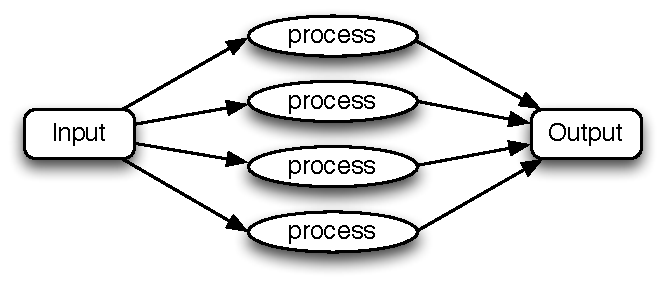
\includegraphics[width=3in]{figs/overview}
%  \caption{A high-level architecture of our approach}
%  \label{fig:overview}
%\end{figure}
